\documentclass[12pt,a4paper]{article}
\usepackage[utf8]{inputenc}
\usepackage[spanish]{babel}
\usepackage{amsmath}
\usepackage{amsfonts}
\usepackage{amssymb}
\usepackage{makeidx}
\usepackage{graphicx}
\usepackage{lmodern}
\usepackage{kpfonts}
\usepackage{fourier}
\usepackage[left=2cm,right=2cm,top=2cm,bottom=2cm]{geometry}
\usepackage[hidelinks]{hyperref}
\author{Luis Angel Torres Pinto }
\title{Operación de los circuitos de activación con tiristores  en convertidores CA-CD y CA-CA}
\begin{document}
\maketitle
\centering

\includegraphics[width=0.8\textwidth]{upzmg.jpg} 

\newpage
\raggedright
\chapter{¿Que son los tiristores?}
El tiristor es un semiconductor de potencia que se utiliza como interruptor, ya sea para conducir o interrumpir la corriente eléctrica, a este componente se le conoce como de potencia por que se utilizan para manejar grandes cantidades de corriente y voltaje, a comparación de los otros semiconductores que manejan cantidades relativamente bajas.\\
\centering
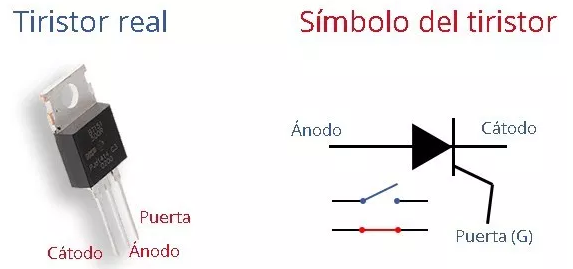
\includegraphics[scale=.50]{tiristores.png}\\
\raggedright
Los tiristores están conformados por 3 terminales un ánodo, un cátodo y una compuerta o mejor conocida “gate”, su funcionamiento se asemeja al de un relevador o un interruptor mecánico, ya que cuando aplicas una corriente a la terminal gate este se activa y obtiene la característica de dejar pasar a la electricidad.\\
\centering
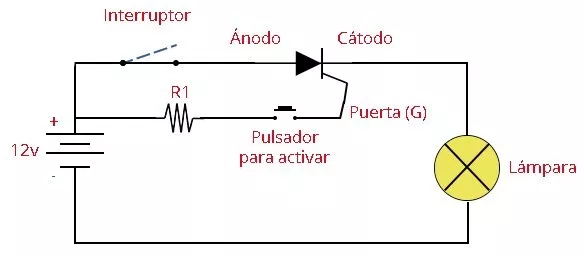
\includegraphics[scale=.60]{tiristores circuitos.png}\\
\raggedright

\section{CA-CD}
Como sabemo este circuito basicamente lo que hace es rectificar la onda complreta cuya carga puede ser puramente resistiva. El convertido de CA-CD nos proporciona una señal de salida rectificada (casi constante) de valor Vm, donde Vm es igual al valor pico del voltaje de entrada.\\
¿Pero que es lo que pasa cuando agregamos un tiristor a este circuito?
Sirve como interruptor el cual nos permite modificar la forma de la onda de tensión y corriente en la carga en función de sus conexiones y desconexiones, por lo que al estar en un convertidor de CA-CD podriamos modificar la tensión y la potencia que se entrega a CD.\\
Monofásico de Media Onda\\
Es un circuito empleado para eliminar la parte negativa o positiva de una señal de corriente alterna de lleno conducen cuando polarizan inversamente. Además su volytaje es positivo.
\centering
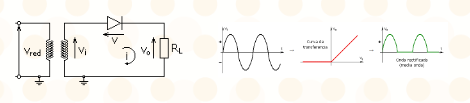
\includegraphics[scale=1]{Monofasico.png} 
\raggedright

\section{CA-CA}
¿Que es lo que pasa cuando un tiristor esta en CA-CA?\\
Durante el semiciclo positivo de la fuente de corriente alterna (c.a.) el ánodo del tiristor es mas positivo que el cátodo y están polarizados directamente. Si ahora le llega una señal suficiente a la puerta el tiristor se activará y pasará corriente de entre ánodo y cátodo. Al principio del ciclo positivo de la onda como no le llega la suficiente corriente a la puerta el tiristor estará desactivado. Llegará un momento que le llegue la suficiente corriente o tensión (tensión de disparo) y es entonces cuando el tiristor se activará. Una parte de la onda no estará en la salida al principio.
\centering
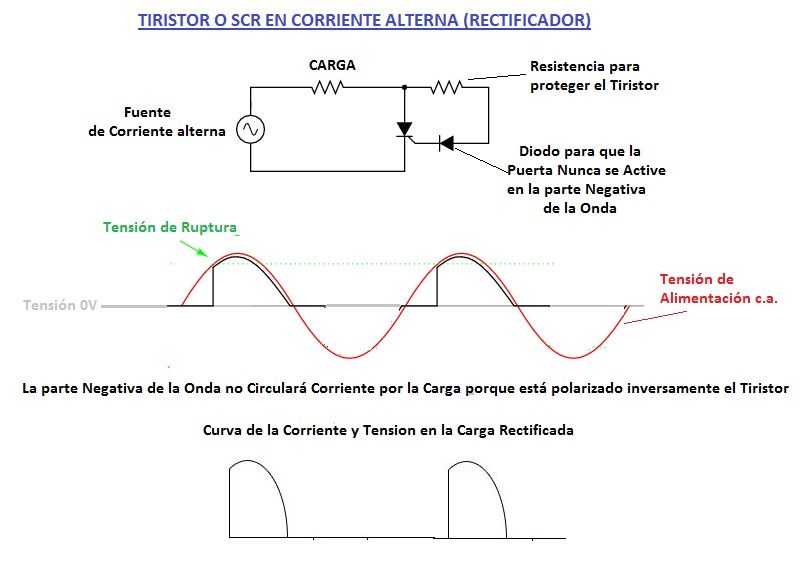
\includegraphics[scale=.60]{alterna.jpg} 
\raggedright
Al pasar por el valor de la corriente de mantenimiento IK, el tiristor se desconecta (sin corriente de salida = interruptor abierto). Durante el otro medio ciclo la polaridad de la fuente es negativa, y esta polaridad hace que el tiristor o SCR quede inversamente polarizado lo cual impide que circule cualquier corriente hacia la carga. Esto significa que no puede estar en conducción por más de medio ciclo. Al volver al ciclo positivo necesitamos activar de nuevo el tiristor con una pequeña corriente en la puerta, pero como está conectada también a la fuente de tensión en alterna, la propia fuente nos la genera.
En la parte de la onda positiva de corriente alterna circula corriente y por la parte negativa no circula corriente, haciendo el tiristor de rectificador, ya que la onda de salida quedaría rectificada (solo la parte positiva).\\
\newpage
\textbf{Referencias}\\
\url{https://www.areatecnologia.com/electronica/tiristor.html}\\
\url{https://www.monografias.com/trabajos105/convertidores-ca-cc-y-ca-ca-tiristores/convertidores-ca-cc-y-ca-ca-tiristores.shtml}\\
\url{https://prezi.com/dh380hlerc_l/convertidores-ca-cd/}\\
\url{http://ccpot.galeon.com/enlaces1737112.html}\\
\url{http://catarina.udlap.mx/u_dl_a/tales/documentos/lem/moyaho_l_i/capitulo1.pdf}
\end{document}